\documentclass[a4paper, oneside, 11pt]{scrbook}

% Get the necessary packages for the document.
% Set to english language and utf8.
\usepackage[english]{babel}
\usepackage[utf8]{inputenc}

% Some packages for symbols we need within the tutorial.
\usepackage{dingbat}
\usepackage{marvosym}

% For the sourcecode.
\usepackage{listings}

% Enable Jan's highlighting
% Usage:
% %% preamble
% \usepackage{listings} %% correct name?
\usepackage{lstide}
% \lstset{tabsize=2,captionpos=b,style=default,}
%
%
% %% main
%     \begin{lstlisting}[style=eclipse-java,gobble=6,caption={Simple micro-benchmark in Java}]
%       for (int i = 0; i < 1000; i++) {
%         tin = currentTime();
%         benchmarkedOperation // testtext
%         tout = currentTime();
%       }
%     \end{lstlisting}

% For the links etc.
\usepackage{hyperref} % avh: removed [pdfborder={0 0 0}]

% For the pdf-graphics.
\usepackage{graphicx}

% The steamroller tactics to fix figures and so on.
\usepackage{float}

% This is for tables which are to long to be shown on one page.
\usepackage{longtable}

% This package is for the directory tree structures
\usepackage{dirtree}
\renewcommand*\DTstylecomment{\footnotesize\normalfont\itshape\rmfamily}
\renewcommand*\DTstyle{\footnotesize\sffamily}

% We need this package for some color within the document.
\usepackage{color}

\usepackage[sort,compress,numbers]{natbib} %round,authoryear

% compactitem, compactenum, ...
\usepackage{paralist}


% This is the package for the margin-nodes.
\usepackage[color=white, bordercolor=white]{todonotes}

\usepackage{amsfonts}
\usepackage{setspace}
\usepackage{ae,aecompl}

\usepackage[automark]{scrpage2}

\usepackage[margin=0.5cm,indention=0em,font={small},labelfont={sf,small},format=hang]{caption}

\usepackage[hang,sf]{subfigure}
\subfigcapmargin=1em

%\usepackage{scrhack}

% Get the new commands we defined for this document.
\newcommand{\Kieker}{\textit{Kieker}}
\newcommand{\home}{$\sim$}


% Set the title and everything.
\titlehead{
	\centering
	\includegraphics[height=25mm]{./images/kieker-logo} \\
	Technische Fakultät \\
	Institut für Informatik \\
	Arbeitsgruppe Software Engineering
}

\title{\Kieker\ Framework\\ \Large{Continuous Monitoring and Analysis of Java Software Behavior}}
\author{Nils Ehmke}
\date{\today}
\subtitle{-- Tutorial --}
\publishers{
%\flushleft

\includegraphics[height=1cm]{./images/cau-sw}
}
% Here we go.
\begin{document}
  % We want a table of contents seperated from the rest of the text.
  \maketitle
  \tableofcontents

  % Insert the other parts of the document.
  \chapter{Introduction}
	\section{What is \Kieker?}

		\Kieker\ is a framework facilitating the monitoring and analysis of control flows, response times and generally the runtime behavior of Java applications. Normal ({}``plain) Java applications can be arranged with the framework as well as server based Java web applications. The framework itself has been developed with regard to providing an easy manageable, maintainable piece of software, which can be included uncomplicated into both, new and existing software projects. Kieker has been designed for a continuous operation, resulting in a very small overhead during the monitoring. Kieker can probe whole method calls as well as single statements (e.g. a = a + 1).\\ 
		Nearly every component of the framework can be extended and adjusted easily as necessary.

		% This is the component diagram of Kieker (the satellite).
		\begin{figure}[H]
			\begin{centering}
				\includegraphics[width=1\textwidth]{images/kiekerComponentDiagram}
			\end{centering}
			\caption{The component diagram of \Kieker}
			\label{Figure:KiekerComponentDiagram}
		\end{figure}
		
		Figure \ref{Figure:KiekerComponentDiagram} shows that the framework consists mainly of two big parts:
		\begin{itemize}
			% Both items get notify-tags because of the important information in here.
			\item \KiekerMonitoringPart\\
			This is the part which is responsible for probing, logging and recording the program behavior. Its core is the singleton class \class{MonitoringController} \notify which receives the records and stores them into different monitoring logs, like for example into files or into databases.
			\item \KiekerAnalysisPart\\
			This part is responsible for the evalution and possible visualization of the recorded information. Its core is the class \class{AnalysisInstance} \notify which manages the lifecycle of the readers and all plugins which shoud analyze the stored informations.
		\end{itemize}
		Both parts are composed of subcomponents which can just be used or extended as well with own classes. The rough interaction between the components is described in Figure \ref{Figure:KiekerCommunicationDiagram} but will be explained furthermore in the course of this tutorial.

		% This image shows the communication diagram of the different components.
		\begin{figure}[H]
			\begin{centering}
				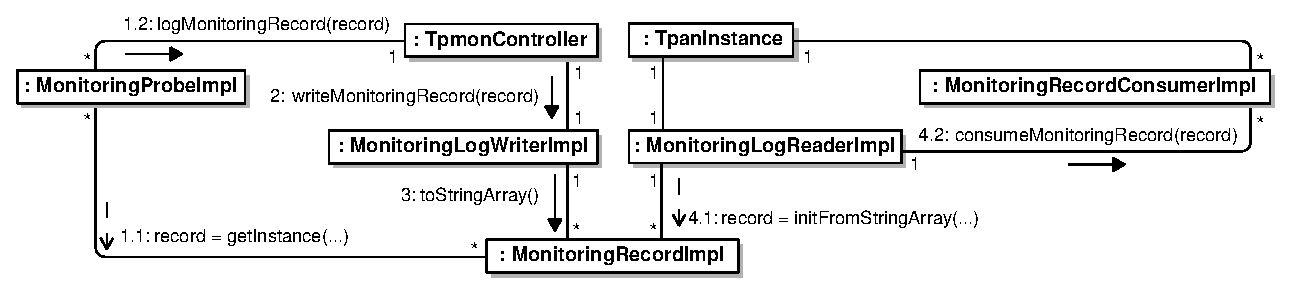
\includegraphics[width=1\textwidth]{images/kiekerCommunications-revisedReArranged-woMonitoringLog-bw}
			\end{centering}
			\caption{The communication diagram of \Kieker}
			\label{Figure:KiekerCommunicationDiagram}
		\end{figure}
		
		% Notify-tag because it is explained how Kieker works.
		\notify The monitoring probes create the monitoring records and deliver them to the monitoring controller. The monitoring controller uses the monitoring log writers to persist the given records which can later be read by a monitoring log reader who creates a monitoring record again. These records can then be used by the consumers in nearly every way.

	\section{Features}
	% This part has to be filled!
	
	\section{The purpose of this tutorial}
		% Short explanation what the tutorial will show now.
		This tutorial will take a closer look at both, the \KiekerMonitoringPart - and the \KiekerAnalysisPart-part. It will be described on the one hand how \KiekerMonitoringPart  can be used to mark parts of the own sourcecode for \Kieker\  and to let them run under surveilance, so that the recorded informations can be persisted somewhere and on the other hand \KiekerAnalysisPart will be used for processing the recorded data.\\
		Before this tutorial goes deeper into the single parts of the framework, it shows how to create and execute a simple example.
  \chapter{Example}
	% A little explanation beforehand
    This chapter will show how to develop a simple example by installing \Kieker\ before marking some code lines for the monitoring. After the necessary data has been collected, they will be analyzed by an own developed component. The example itself is available on the website of \Kieker.
	
	\section{Download and Installation}
      \Kieker\ can be downloaded from \KiekerDownloadUrl. The content of the zip- respectively the tar.gz-file should be extracted to any directory, which we will call ``\KiekerDir`` within this tutorial. The installation of \Kieker\ is completed.\\
      If desired, the new created path can of course be assigned to an easy remindable environment variable. 
 
    \section{Monitoring}
      For the creation of the example it is recommended to create a new working directory (e.g. ''example'') of the following structure:
      \begin{center}
		  \dirtree{%
		  .1 example\DTcomment{The root directory of the project}.
		  .2 build\DTcomment{The directory for the compiled class files for Java}.
		  .2 lib\DTcomment{The directory for the libraries and needed jar-files}.
		  .3 \monitoringCtrlJar\DTcomment{}.
		  .3 \commonJar\DTcomment{}.
		  .3 commons-logging-1.1.1.jar\DTcomment{}.
		  .2 src\DTcomment{The directory for the sourcecode files}.
		  .3 mySimpleKiekerExampleManual\DTcomment{The directory for the new package}.
		  .4 CRM.java\DTcomment{One of the sourcecode files}.
		  .4 Catalog.java\DTcomment{One of the sourcecode files}.
		  .4 Bookstore.java\DTcomment{One of the sourcecode files}.
		  .4 BookstoreStarter.java\DTcomment{One of the sourcecode files}.
		  }      
      \end{center}
	  The listed jar-files must be copied from the \Kieker\ directory:
      \begin{itemize}
		\item \KiekerDir/dist/\commonJar\
		\item \KiekerDir/dist/\monitoringCtrlJar\
		\item \KiekerDir/lib/commons-logging-1.1.1.jar
      \end{itemize}
      The sourcecode files consist of the following lines:
      % It isn't necessary to do this every time but it makes sure that the listing has the correct format.
      \setJavaCodeListing

	  % If the Path to the examples changes, then they have to be changed here AS WELL!!
      \lstinputlisting[caption=Bookstore.java]{source-example/manual-monitoring/src/mySimpleKiekerExampleManual/Bookstore.java}

	  % Due to this package we have to write the important part manually...
	  \begin{lstlisting}[caption=BookstoreStarter.java]
		package mySimpleKiekerExampleManual;

		import kieker.analysis.plugin.MonitoringRecordConsumerException;
		import kieker.analysis.reader.MonitoringLogReaderException;

		public class BookstoreStarter {
			public static void main(String[] args) throws MonitoringLogReaderException,
				MonitoringRecordConsumerException {
				/* Start the monitoring */
				Bookstore.startBookstoreRequests();
			}

		}
	  \end{lstlisting}
	  
      \lstinputlisting[caption=CRM.java]{source-example/manual-monitoring/src/mySimpleKiekerExampleManual/CRM.java}

      \lstinputlisting[caption=Catalog.java]{source-example/manual-monitoring/src/mySimpleKiekerExampleManual/Catalog.java}
	  
      The monitoring itself is done manually. Although this is not the strength of \Kieker\ it is pretty good for a quick start.
	  
      % Make sure that this listing will be modified, once the sourcecode changes!!! 
	  % It must show the whole monitoring of the bookstorecall, from getting the first time to persisting of the record!!
      \lstinputlisting[firstline=20, lastline=29, caption=Cutting from Bookstore.java, label=listing:cuttingBookstore]{source-example/manual-monitoring/src/mySimpleKiekerExampleManual/Bookstore.java}
	  
      In Listing \ref{listing:cuttingBookstore} can be seen, how the monitoring itself is done. We remember the time before and after a specific method call (in this case: \textit{searchBook()}). These informations are stored in the so called operation execution record. Its (partially) layout can be seen in Figure \ref{image:operationexecutionrecordclassdiagram}.
	  
	  % This figure contains the short class diagram of the operation execution record.
		\begin{figure}[H]
			\begin{center}
				%\includegraphics[width=1.0\textwidth]{}
				\caption{The class diagram of the operation execution record}
				\label{image:operationexecutionrecordclassdiagram}
			\end{center}
		\end{figure}
	  
		The important attributes are:
		\begin{itemize}
			\item The component (the class) in which the called method is.
			\item The called method.
			\item The trace id of the current trace we want to record. Due to the fact, that we follow only one trace, this is zero in all recordings.
			\item The time before the sourcecode which should be measured.
			\item The time after the sourcecode which should be measured.
		\end{itemize}
		  
		The sourcecode should now be compilable and executable:
		
		% We need something like the ouput from the bash.
		
		\setBashListing
		% Note: This is different under Windows and Linux!!
		% If the Kieker-Dir for the tutorial is changed, make sure that this is done here as well!!
		% We cannot put a latex-macro within the listing!
		\begin{lstlisting}
			nils@Laptop:~/example$ javac src/mySimpleKiekerExampleManual/*.java\
			-classpath\
			./lib/kieker-common-1.5-trunk.jar:\
			./lib/kieker-monitoring-1.5-trunk.jar:\
			-d build

			nils@Laptop:~/example$ java -Dlog4j.configuration=$<$KIEKER-DIR$>$/META-INF/log4j.properties\
			-classpath\
			./build/:\
			./lib/kieker-common-1.5-trunk.jar:\
			./lib/kieker-monitoring-1.5-trunk.jar:\
			./lib/commons-logging-1.1.1.jar\
			mySimpleKiekerExampleManual.BookstoreStarter
		\end{lstlisting}
		If the sourcecode should be compiled and executed under Windows, the paths have do be sepereated with semicolons instead of colons. Furthermore it is not possible to wrap the single parts of the commands with a backslash.\\
		If everything worked correctly, there should now be a new directory named ``tpmon-20100605-115948636-UTC'' (just with other numbers) in the default temporary directory (under Linux this should be ``/tmp''; under Windows ``C:/temp''). In this directory, there should be a file with the extension ``.dat'' which contains the recorded informations from the source code. A possible content of this file can be found in the appendix of this tutorial.\\
		Now we take a closer look at the analysis.

	\section{Analysis}
      % Here we go...we have to inform the user of the programs he need for the converting. And that means as well, that a window user cannot do this part.
      For the visualization via \Kieker\ we need the both tools graphviz (\url{www.graphviz.org/}) and plotutils (\url{www.gnu.org/software/plotutils/}).\\
      Assume that we already have our recorded informations saved in a ``.dat''-file somewhere for example in the ``tmp``-directory, we can now start with converting these informations into graphs. For the first, we change into our \Kieker\-directory ($\sim$/kieker). It is recommended to create a new directory for the graphs first:
      \begin{lstlisting}
	nils@Laptop:~/kieker$ mkdir /tmp/graphs
      \end{lstlisting}
      The shell-script ''./bin/trace-analysis.sh`` will now do most of the job. It starts the analysis and uses the above-mentioned tools to convert to files into graphs and diagrams.
      \begin{lstlisting}
	nils@Laptop:~/kieker$ ./bin/trace-analysis.sh --plot-Sequence-Diagrams --short-labels -i /tmp/tpmon-20100606-112536844-UTC/ -o /tmp/graphs/
      \end{lstlisting}
	The command ''--plot-Sequence-Diagrams`` tells the shell script to convert our data into a sequence diagram\footnote{Other diagrams and graphs can be plot of course as well. Start trace-analysis.sh without any parameters to see the possible commands.}; with ''--short-labels`` we make sure that the components get a shorter name and the directories after ''-i`` and ''-o`` are the input- and the output-directories. If everything went well, \Kieker\ converted the data into files, which can now converted directly into visual graphs:
	\begin{lstlisting}
	  nils@Laptop:~/kieker$ ./bin/dotPic-fileConverter.sh /tmp/graphs/ svg
	\end{lstlisting}
	The shell script ''./bin/dotPic-fileConverter.sh`` gets the directory with the files and the desired file extension (e.g. svg or png). The resulting graphs should now be available in ''/tmp/graphs`` and should look like figure \ref{image:sequencediagram}
	% This is the simple sequence diagram which results by running the bookstore example; of course without showing the traces etc.
	\begin{figure}[H]
	  \begin{center}
	    \includegraphics[width=0.7\textwidth]{sequenceDiagram.pdf}
            \caption{The resulting sequence diagram}
	    \label{image:sequencediagram}
	  \end{center}
	\end{figure}
	We are now able to monitor source code and to visualize these recorded informations in a simple way.

    \section{Using AOP}
      Now we want to monitor whole methods without surrounding the method calls with a block where we keep the time manually. We will now use so called annotations to mark the methods we want to monitor\footnote{To be more precisely: We use annotations which will then be used by the aspect-oriented Java extension named AspectJ to surround the method calls with code blocks which are similar to these, we already used manually.}. As can be seen in the following listing we write the annotation \textit{kieker.monitoring.annotation.TpmonExecutionMonitoringProbe} above the methods to be monitored. 
      \setJavaCodeListing
      \lstset{caption=Bookstore.java, label=listing:Bookstore2.java}
      \lstinputlisting{source-example/annotation-monitoring/src/mySimpleKiekerExample/bookstoreTracing/Bookstore.java}
      Due to the use of AspectJ we need now to copy the file ''META-INF/aop.xml.example`` from our \Kieker\ directory to our working directory to ''META-INF/aop.xml``. This file tells AspectJ which parts of our source code should be monitored. To inform AspectJ about our own annotations, we need another libarary as well. We copy $\sim$/kieker/dist/kieker-tpmon-\version\_ctw.jar to our own example project in $\sim$/example/lib/kieker-tpmon-\version\_ctw.jar\\
      To make sure that every method in our program which is annotated will be monitored, we have to write the following into the ''aop.xml``:
      \setXMLListing 
      \begin{lstlisting}
	<aspectj>
	  <!-- turn verbose on to check which files are instrumented -->
	  <!-- <weaver options="-verbose"/> -->
	  <weaver options="">
	      
	  <!-- The following line is the important one -->
	  <include within="*"/> 

	  <!-- uncomment following to instrument sun jpetstore -->
      \end{lstlisting}
      The compiling is pretty much the same as before (except for some more libraries), but in order to run the program, we have to copy the configuration files into the build-directory.
      % Same as before. If the libraries change, this has to be modified as well.
      \begin{lstlisting}
	nils@Laptop:~/example$ javac ./src/mySimpleKiekerExample/bookstoreTracing/Bookstore.java ./src/mySimpleKiekerExample/bookstoreTracing/Catalog.java ./src/mySimpleKiekerExample/bookstoreTracing/CRM.java -classpath ./lib/kieker-monitoring-1.5-trunk_ctrl.jar:./lib/commons-logging-1.1.1.jar -d build/
	nils@Laptop:~/example$ cp -r ./META-INF/ ./build/META-INF
	nils@Laptop:~/example$ java -Dlog4j.configuration=META-INF/log4j.properties -javaagent:lib/aspectjweaver-1.6.6.jar -Dorg.aspectj.weaver.showWeaveInfo=true -Daj.weaving.verbose=true -classpath ./build/:./lib/kieker-monitoring-1.5-trunk_ctrl.jar:./lib/commons-logging-1.1.1.jar:./lib/kieker-monitoring-1.5-trunk_ctw.jar mySimpleKiekerExample.bookstoreTracing.Bookstore
      \end{lstlisting}
    \chapter{\KiekerMonitoring}
    \section{Configuration}
      The monitoring part of \Kieker\ can be configured using the configuration file named ''\monitoringPropertiesFile``. This file should be copied for use to the directory ''META-INF`` of the own project and should - like the ''aop.xml`` - be copied during compiling. In order to inform \Kieker\ about this file, the following parameter should be used for the JVM:
      \begin{lstlisting}
	-Dkieker.monitoring.properties=META-INF/kieker.monitoring.properties
      \end{lstlisting}
      Most of the variables are self-explanatory and some of them will be explained in the following.

    \section{Records}
      % They are not really only part of the monitoring components, but they have to be mentioned somehow.
      As we already saw, the records are the objects which store the monitored informations somehow. They are not really part of \KiekerMonitoring\ but in order to the use in the following, we will examine them.\\
      If we want to implement an own record, it should be extend the already existing class \textit{kieker.common.record.AbstractMonitoringRecord}. The record should be able to put his complete content into an array (of Object] so that the other components of \Kieker\ are able to persist and load the data and should of course provide a method to restore the content from an array. The following listing shows a simple record implementation which has fields for the class and the method that is called.
      \setJavaCodeListing
      \lstset{caption=MyRecord.java}
      \lstinputlisting{source-example/monitoring-and-analysis-with-own-components/src/mySimpleKiekerExample/bookstoreTracing/MyRecord.java}

    \section{Probes}
      The probes are responsible for the decision which (and where) informations should be recorded. Technically we already implemented them by surrounding the method calls with the correct statements to clock, to produce the records and to deliver these records to the monitoring controller. Other specific controller could for example record only the amount of delivered bytes between methods or record only every second method call as well.\\
      We already used the annotations to make the monitoring much more comfortable and could also implement own annotations for AspectJ, but this won't be explained in this tutorial, because it would simply go beyond the scope.

    \section{Writers}
      \hypertarget{monitoringlogwriters} 
      The so called \textit{monitoring log writers} (they can be seen as well in figure \ref{image:kiekercomponentdiagram}) are the parts of \Kieker\ which are responsible for writing and serializing the recorded informations into files, databases and so on. In other words: They get an instance of \textit{AbstractKiekerMonitoringRecord} and produce an output of any nature whatsoever.\\
      Of course there are already some writers implemented, as can be seen in figure \ref{image:writers}.
      % This is the diagram with the different types of writers.
      \begin{figure}[H]
	\begin{center}
	  \includegraphics[width=0.5\textwidth]{kieker_writerimpls.pdf}
	  \caption{The inheritance hierarchy of the current implemented monitoring log writers}
	  \label{image:writers}
	\end{center}
      \end{figure}
      As the quick start part already showed it, every monitored record is sent to the \textit{TpmonController} which itself calls the current writer. The writer uses for example the \textit{toArray()} method of the record to get the informations stored by the record as handable array. The writer is then able to write these objects for example into a file.\\
      The implementation of an own writer class is quiet simple and can be done by implementing the interface \textit{kieker.monitoring.writer.IMonitoringLogWriter}. The following listing shows an example writer which uses a named pipe\footnote{The class \textit{MyNamedPipeManager} will be shown in the appendix of this tutorial.} to write the given records directly into the memory.
      \setJavaCodeListing
      \lstset{caption=MyWriter.java}
      \lstinputlisting{source-example/monitoring-and-analysis-with-own-components/src/mySimpleKiekerExample/bookstoreTracing/MyWriter.java}
      It is necessary to tell \KiekerMonitoring\ which writer should be used. This can be done in the already mentioned file ''\monitoringPropertiesFile``:
      \setBashListing
      \begin{lstlisting}
	monitoringDataWriter=mySimpleKiekerExample.bookstoreTracing.MyWriter
	monitoringDataWriterInitString=somePipe

	# 1.1.5 [property has been removed:] Use monitoring record type IDs

	# 1.1.6 Queue Size used to store Monitoring Records
	# Asyncronous Writers need to store Monitoring Records in an internal Queue.
	# This parameter defines the Number of Records cached. If this number is exceeded
	# Kieker will terminate with a Queue Full Exception!
	#
	asyncRecordQueueSize=8000
      \end{lstlisting}
      The first property decides which writer should be used. If we don't use any of the already implemented writers, we have to deliver the whole name of the class of the writer. The second property is an init string which can be used to initialize the writer in any way. In this case we use this parameter to tell the writer which pipe should be used. The third property is just important for asyncronous writers. It must be pointed out that the resulting init string our writer gets is of the form ''somePipe $|$ asyncRecordQueueSize=8000``. 
  \chapter{\Kieker\ Analysis Component}
      % The analysis works a little bit different, that is why we explain it here.
      \KiekerAnalysis\ is the part of \Kieker\ which is responsible for the analysis, consisting of the reader, the consumer and the analysis instance itself. After we stored somewhere our records, we need to read them again somehow. This is task of the reader. Whatever we want to do with these informations is task of the consumers. They can for example evaluate, process or visualize the data. The analysis instance concerns about the lifetime and registration of the other parts.\\
      The analysis consists roughly of the following steps:
      \begin{enumerate}
	\item Create one (or more) analysis instance.
	\item Set the reader of this instance and line it with the necessary informations to read the stored records.
	\item Register the consumers who should do something with the recorded data.
	\item Start the analysis instance.
      \end{enumerate}
      % For the moment we don't have ANY configuration for the analysis part. This has to be done in the program.
      % \section{Configuration}

      \section{Readers}
	The \textit{monitoring log readers} (their position can be found in figure \ref{image:kiekercomponentdiagram}) are the direct counterpart to the \hyperlink{monitoringlogwriters}{\textit{monitoring log writers}}. While the writers get a record and write them in files or somewhere else, the readers take the writen data (from files, databases and so on) and convert them into a suitable instance of \textit{AbstractKiekerMonitoringRecord}. That means, that whenever we are implementing a new writer, we should also implement a corresponding reader. If we want for example save our recorded informations in a database, we have to be capable of reading these stored informations from the database again.\\
	Again there are some readers already implemented in \Kieker\ but we can implement an own reader as well. The following diagram shows the rough hierarchy.
	% This is the diagram with a simple reader hierarchy.
	\begin{figure}[H]
	  \begin{center}
	    \includegraphics[width=0.5\textwidth]{kieker_readerimpls.pdf}
	    \caption{The simple inheritance hierarchy of some currently implemented monitoring log readers}
	    \label{image:readers}
	  \end{center}
	\end{figure}
	The implementing of an own reader is nearly the same as the implementing of the writer, but to keep things simple, it is recommended to extend the already implemented AbstractKiekerMonitoringLogReader, because otherwise it would be necessary to implement the used observer pattern of the reader. By using the methods of the abstract class \textit{kieker.analysis.reader.AbstractMonitoringLogReader}, the task of delivering a new record to the consumers can be delegated to the super class.\\
	The following listing shows a simple reader which reads a stored record from the pipe. If there is nothing on the pipe to be read, the reader waits 4 seconds at maximum before it terminates.
	\setJavaCodeListing
	\lstset{caption=MyReader.java}
	\lstinputlisting{source-example/monitoring-and-analysis-with-own-components/src/mySimpleKiekerExample/bookstoreTracing/MyReader.java}

      \section{Consumers}
	The consumers are the parts of \Kieker\ which work with the records that have been loaded by the reader. There can be (theoretically) an infinite number of consumers which produce any kind of output. A consumer can be programmed by implementing the interface \textit{kieker.analysis.plugin.IMonitoringRecordConsumerPlugin} and implementing the necessary methods. Our following example consumer takes the given record and writes the content to the default output stream.
	\setJavaCodeListing
	\lstset{caption=MyConsumer.java}
	\lstinputlisting{source-example/monitoring-and-analysis-with-own-components/src/mySimpleKiekerExample/bookstoreTracing/MyConsumer.java}

      \section{The analysis}
	To put everything together, the following listing shows how to use the above-mentioned components.
	% It is not necessary to show the whole method.
	\setJavaCodeListing
	\begin{lstlisting}
	  AnalysisInstance ai = new AnalysisInstance();
	  MyReader reader = new MyReader();
	  reader.init("somePipe");
	  ai.setLogReader(reader);
	  ai.registerPlugin(new MyConsumer());
	  ai.run();
	\end{lstlisting}
  \chapter{Trace Analysis and Monitoring}
  %%%%%%%%%%%%%%%%%%%%%%%%%%%%%%%%%%%%%%%%%
% Appendix
% 
% $Date$
% $Rev$:
% $Author$


\appendix

\chapter*{Appendix}\label{appendix}
\addcontentsline{toc}{chapter}{Appendix}
\addtocontents{toc}{\protect\setcounter{tocdepth}{-1}}

\chapter{Wrapper scripts}\label{appendix:wrapperScripts}
The \dir{bin/} directory of \Kieker's binary release contains some \file{.sh}  and %
\file{.bat} scripts to invoke tools included in \file{\mainJar{}}. %
The following sections give a short description of their functionality and %
list their usage outputs as printed to the standard output stream when %
called without command-line parameters. %
In addition to the standard output stream, the file \file{kieker.log} %
is used for logging output during execution.

% generated by the script gen-bin-usage-tex.sh with manual adjustments

\section{Script \file{convertLoggingTimestamp.sh|bat}}

The script converts \KiekerMonitoringPart{} logging timestamps, %
representing the number of nanoseconds since 1~Jan 1970 00:00 UTC, to a %
human-readable textual representation. %

\

\noindent Main-class: {\small \class{kieker.tools.loggingTimestampConverter.LoggingTimestampConverterTool}}

\paragraph*{Usage}\

\setTextListing
\lstinputlisting[caption=]{Appendix-usage-convertLoggingTimestamp.sh.inc}

\paragraph*{Example}\

\setTextListing
\begin{lstlisting}
$\lstshellprompt{}$ $\textbf{bin/convertLoggingTimestamp.sh}$ $\textbf{-t}$ 1283156545581511026 1283156546127117246 
1283156545581511026: Mo, 30 Aug 2010 08:22:25 +0000 (UTC) (Mo, 30 Aug 2010 10:22:25 +0200 (local time))
1283156546127117246: Mo, 30 Aug 2010 08:22:26 +0000 (UTC) (Mo, 30 Aug 2010 10:22:26 +0200 (local time))
\end{lstlisting}

\section{Script \file{logReplay.sh|bat}}

Replays filesystem monitoring logs created by \KiekerMonitoringPart{}. %
Example applications are:
\begin{compactitem}
\item Merging multiple directories containing monitoring data into a single %
output directory. 
\item Importing a filesystem monitoring log to another monitoring log, e.g., %
a database. Therefore, an appropriate \KiekerMonitoringPart{} configuration %
file must be passed to the script (see Section~\ref{sec:monitoring:configuration}).
\item Replaying a recorded filesystem monitoring log in real-time in order to simulate %
incoming monitoring data from a running system, e.g., via JMS~(see also Appendix~\ref{appendix:usingJMS}). 
\end{compactitem}

\

\noindent Main-class: {\small \class{kieker.tools.logReplayer.FilesystemLogReplayerStarter}}

\paragraph*{Usage}\

\setTextListing
\lstinputlisting[caption=]{Appendix-usage-logReplay.sh.inc}

\paragraph*{Example}\

\noindent The following command replays the monitoring testdata included in %
the binary release to another directory:

\setTextListing
\begin{lstlisting}
$\lstshellprompt{}$ $\textbf{bin/logReplay.sh}$
  $\textbf{--inputdirs}$ $\distributedTestdataDirDistro$ 
  $\textbf{--keep-logging-timestamps}$ $true$ 
  $\textbf{--realtime}$ $false$
\end{lstlisting}

\section{Script \file{trace-analysis.sh|bat}}

\paragraph*{Usage}\

\setTextListing
\lstinputlisting[caption=]{Appendix-usage-trace-analysis.sh.inc}

\paragraph*{Example}\

Examples on using this script can be found in Chapter~\ref{chap:aspectJ} and %
Appendix~\ref{appendix:traceAnalysisOutputExamples}.

\chapter{\KiekerMonitoringPart{} Configuration File}\label{sec:appdx:monitoringproperties}

This is the file \file{\monitoringPropertiesFile} from the binary release and 
constitutes \KiekerMonitoringPart{}'s default configuration.

\

\setXMLListing
\lstinputlisting[caption=\monitoringPropertiesFile]{../../META-INF/kieker.monitoring.properties}

\section{Script \file{dotPic-fileConverter.sh|bat}}

\paragraph*{Usage \& Example}\

\setTextListing
\lstinputlisting[caption=,firstline=3]{Appendix-usage-dotPic-fileConverter.sh.inc}



\chapter{\KiekerMonitoringPart{} Default Configuration}\label{sec:appdx:monitoringproperties}
This is the file \file{\monitoringPropertiesFile} from the binary release and 
constitutes \KickerMonitoringPart{}'s default configuration. %
Section~\ref{sec:monitoring:configuration} describes how to use a custom configuration.

\

\setPropertiesListing
\lstinputlisting[caption=\monitoringPropertiesFile]{../../src/monitoring/META-INF/kicker.monitoring.default.properties}


\chapter{Additional Source Code Listings}\label{appendix:additionalSourceCode}
\section{MyNamedPipeManager and MyPipe}\label{appendix:pipeListings}

\enlargethispage{1cm}

      \setJavaCodeListing
      \lstinputlisting[firstline=21, firstnumber=21,caption=MyNamedPipeManager.java]{\customComponentsBookstoreApplicationDir/src/bookstoreApplication/MyNamedPipeManager.java}
\newpage
      \setJavaCodeListing
      \lstinputlisting[firstline=21, firstnumber=21, caption=MyPipe.java]{\customComponentsBookstoreApplicationDir/src/bookstoreApplication/MyPipe.java}
      
      \setJavaCodeListing
      \lstinputlisting[firstline=21, firstnumber=21, caption=PipeData.java]{\customComponentsBookstoreApplicationDir/src/bookstoreApplication/PipeData.java}

\chapter{Example Console Outputs}\label{appendix:exampleConsoleOutputs}
\section{Quick Start Example (Chapter~\ref{chap:example})}\label{sec:appendix:manualInstrumentation:output}
% \subsubsection{Monitoring}
% 		The following listing shows the produced log during a run of the Bookstore Application with the manual monitoring probes.
\setTextListing
\lstinputlisting[caption=Execution of the manually instrumented Bookstore application (Section~\ref{sec:example:monitoring})]
{ch2-quickstart-example/kieker-20120402-163314855-UTC-myHost-KIEKER-SINGLETON-monitoring.stdout}
\newpage
% \subsubsection{Analysis}
% 		The second listing is the log during the analysis of the produced data. It can be seen that some of the calls are accepted and some others refused.
\setTextListing
\lstinputlisting[caption=Execution of the example analysis (Section~\ref{sec:example:analysis})]
{ch2-quickstart-example/kieker-20130910-120352847-UTC-myHost-KIEKER-SINGLETON-analysis.stdout}
\newpage	
\section{Trace Monitoring, Analysis \& Visualization (Chapter \ref{chap:aspectJ})}%
\label{sec:appendix:exampleConsoleOutputs:aspectJExample}
\setTextListing
\begin{lstlisting}[caption=Execution of the Bookstore with AspectJ trace instrumentation (Section~\ref{sec:traceAnalysis:instr:AspectJ})]
Bookstore.main: Starting request 0
10.04.2012 13:03:51 kieker.monitoring.core.configuration.ConfigurationFactory createSingletonConfiguration
INFO: Loading properties from properties file in classpath: 'META-INF/kieker.monitoring.properties'
10.04.2012 13:03:51 kieker.monitoring.core.controller.MonitoringController createInstance
INFO: Current State of kieker.monitoring (1.5) Status: 'enabled'
        Name: 'KIEKER'; Hostname: 'pc-vanhoorn'; experimentID: '1'
JMXController: JMX disabled
RegistryController: 0 strings registered.
TimeSource: 'kieker.monitoring.timer.SystemNanoTimer'
        Time in nanoseconds (with nanoseconds precision) since Thu Jan 01 01:00:00 CET 1970'
WriterController:
        Number of Inserts: '0'
        Automatic assignment of logging timestamps: 'true'
Writer: 'kieker.monitoring.writer.filesystem.AsyncFsWriter'
        Configuration:
                kieker.monitoring.writer.filesystem.AsyncFsWriter.QueueFullBehavior='0'
                kieker.monitoring.writer.filesystem.AsyncFsWriter.flush='true'
                kieker.monitoring.writer.filesystem.AsyncFsWriter.QueueSize='10000'
                kieker.monitoring.writer.filesystem.AsyncFsWriter.customStoragePath='.'
                kieker.monitoring.writer.filesystem.AsyncFsWriter.MaxShutdownDelay='-1'
                kieker.monitoring.writer.filesystem.AsyncFsWriter.storeInJavaIoTmpdir='true'
                kieker.monitoring.writer.filesystem.AsyncFsWriter.maxEntriesInFile='25000'
        Records lost: 0
        Writer Threads (1): 
                Finished: 'false'; Writing to Directory: '/tmp/kieker-20110428-142829399-UTC-Kaapstad-KIEKER'
Sampling Controller: Periodic Sensor available: Current Poolsize: '0'; Scheduled Tasks: '0'

10.04.2012 13:03:51 kieker.monitoring.core.registry.ControlFlowRegistry <clinit>
INFO: First threadId will be 7752665283541598209
10.04.2012 13:03:51 kieker.monitoring.core.controller.MonitoringController$\$$1 run
INFO: ShutdownHook notifies controller to initiate shutdown
10.04.2012 13:03:51 kieker.monitoring.core.controller.MonitoringController cleanup
INFO: Shutting down Monitoring Controller (KIEKER)
10.04.2012 13:03:51 kieker.monitoring.writer.AbstractAsyncWriter terminate
INFO: Shutting down writers.
\end{lstlisting}




\chapter{Ant Scripts}\label{appendix:antScripts}
\section{Quick Start Example (Chapter \ref{chap:example})}
The following \file{build.xml} and \file{build.properties} files can be %
used for compiling and executing the manually instrumentated Bookstore %
application and the analysis, as described in Chapter~\ref{chap:example}. %
The files are included in the directory \file{\manualInstrumentedBookstoreApplicationDirDistro{}/}.

      In order to run the analysis of the application, it is necessary to pass the location of the monitoring log directory. This is done via the parameter \textit{analysis.directory}, e.g.:
      \setBashListing
      \begin{lstlisting}[caption=Command to compile and run the instrumented Bookstore via ant]
#\lstshellprompt{}# ant run-analysis -Danalysis.directory /tmp/kieker-20120402-163314855-UTC-myHost-KIEKER-SINGLETON
\end{lstlisting}%-KIEKER


% \enlargethispage{1.2cm}
      \setPropertiesListing
      \lstinputlisting[caption=build.properties]{\manualInstrumentedBookstoreApplicationDir/build.properties}
      \setAntListing
      \lstinputlisting[caption=build.xml]{\manualInstrumentedBookstoreApplicationDir/build.xml}
\newpage
\section{Custom Components (Chapters \ref{chap:componentsMonitoring} and \ref{chap:componentsAnalysis})}
      The following \file{build.xml} and \file{build.properties} files can be used for compiling and executing the manually instrumentated Bookstore application with the custom components, as described in Chapters~\ref{chap:componentsMonitoring} and \ref{chap:componentsAnalysis}. %
The files are included in the directory \file{\customComponentsBookstoreApplicationDirDistro{}/}.
      \setPropertiesListing
      \lstinputlisting[caption=build.properties]{\customComponentsBookstoreApplicationDir/build.properties}
      \setAntListing
      \lstinputlisting[caption=build.xml]{\customComponentsBookstoreApplicationDir/build.xml}
\newpage
\section{AspectJ-based Trace Monitoring (Chapter \ref{chap:aspectJ})}
      The following \file{build.xml} and \file{build.properties} files can be used for compiling and executing the Bookstore application instrumentated with AspectJ (see Chapter~\ref{chap:aspectJ}). %
The files are included in the directory \file{\aspectJBookstoreApplicationDirDistro{}/}.
\vspace{-3ex}
      \setPropertiesListing
      \lstinputlisting[caption=build.properties]{\aspectJBookstoreApplicationDir/build.properties}     
\enlargethispage{1.1cm}
      \setAntListing
      \lstinputlisting[caption=build.xml]{\aspectJBookstoreApplicationDir/build.xml}

\chapter{Java~EE Servlet Container Example}\label{appendix:JavaEEServletExample}
The \Kieker{} download site\footnote{\KiekerDownloadURL{}} includes an additional %
example \file{\JavaEEServletExampleName}. Using the sample Java Web application %
iBATIS JPetStore\footnote{\url{http://ibatis.apache.org/}}, this example %
demonstrates how to employ \KiekerMonitoringPart{} for monitoring a Java application %
running in a Java~EE container---in this case, Apache Tomcat\footnote{\url{http://tomcat.apache.org/}}. %
Monitoring probes based on the Java~EE Servlet API %
and AspectJ are used to monitor execution, trace, and session data (see Section~\ref{chap:aspectJ}).

\section{Preparation of the Tomcat Servlet Container}

\begin{compactenum}
\item Copy the files \file{\mainJar}, \file{\commonsLoggingJar}, and \file{\aspectJWeaverJar} from %
\Kieker{}'s binary distribution to the Tomcat's \dir{lib/} directory.
\item Copy the file \file{\servletWar} from \Kieker{}'s %
binary distribution to the Tomcat's \dir{webapps/} directory.
\item Tomcat's \dir{lib/} directory contains the files \file{kieker.monitoring.properties} %
and \file{aop.xml} --- the configuration of \KiekerMonitoringPart{} and the %
AspectJ-based instrumentation. %
\item
 Tomcat's start script \file{bin/catalina.\{sh|bat\}} file was modified to add the location %
of the \file{kieker.\-moni\-toring.properties} and the AspectJ agent to the argument %
list of the JVM call:
\end{compactenum}

\enlargethispage{1cm}

\setPropertiesListing
\lstinputlisting[firstline=188,firstnumber=188,lastline=190,caption={Excerpt from catalina.sh (for \UnixLikeSystems)},numbers=left]{\JavaEEServletExampleDir/Tomcat6.0.18WithJpetStore-withInstrumentedJPetStore/bin/catalina.sh}

\setPropertiesListing
\lstinputlisting[firstline=121,firstnumber=121,lastline=123,caption={Excerpt from catalina.bat (for Windows)},numbers=left]{\JavaEEServletExampleDir/Tomcat6.0.18WithJpetStore-withInstrumentedJPetStore/bin/catalina.bat}

%% BEGIN: Windoof
% set JAVA_HOME=%ProgramFiles%\Java\jdk1.6.0_23
% start bin/startup.bat
%% END: Windoof

\begin{compactenum}\setcounter{enumi}{4}
\item  A prepared \file{jpetstore.war} file is already located in the %
   Tomcat's \dir{webapps/} directory. If you want to rebuild the sources, %
   for example to modify the instrumentation, see Section~\ref{sec:Appendix:JPetStoreExample:rebuild}. 
\end{compactenum}


\section{JPetStore and \KiekerMonitoringPart{} Control Servlet}

\noindent We will now start the Tomcat server and generate some monitoring data by manually %
accessing the JPetStore web application. 

\

\enlargethispage{1.5cm}

\begin{compactenum}
\item Start the Tomcat server using the \file{bin/startup.sh} or \file{bin/startup.bat} (\UnixLikeSystems/Windows) %
   script in the Tomcat's \dir{bin/} directory.

   You should make sure, that the Tomcat started properly, by taking 
   a look at the \file{logs/catalina.out} file, \file{logs/catalina.<date>.log} file respectively. %
   On error, the file \file{logs/localhost.<date>.log} may contain details % 
   to resolve the issue.
\item Now, you can access the JPetStore application by opening the URL
   \url{http://localhost:8080/jpetstore/} (Figure~\ref{fig:jpetstore}). %
   \Kieker{} intialization messages should appear in \file{logs/catalina.out}, \file{logs/catalina.<date>.log} respectively. %
   The output includes the information where the monitoring data is written to
   (should be Tomcat's \dir{temp/kieker-<DATE-TIME>/} directory).
\item  Browse through the application to generate some monitoring data. %
   This data can be analyzed and visualized using \KiekerTraceAnalysis{}, %
   as described in Chapter~\ref{chap:aspectJ}.
\item \Kieker{} includes a servlet to control the status of \KiekerMonitoringPart{}. %
   It can be accessed via \url{http://localhost:8080/kieker-monitoring-servlet-\version/} %
   (Figure~\ref{fig:controlServlet}).
\end{compactenum}

\begin{figure}[h]\centering
\hfill
\subfigure[iBATIS JPetStore]{\label{fig:jpetstore}%
\includegraphics[width=0.45\textwidth]{images/jpetstore-example-FFscrsh}}
\hfill
\subfigure[\KiekerMonitoringPart{} control servlet]{\label{fig:controlServlet}%
\includegraphics[width=0.45\textwidth]{images/kieker-servlet-FFscrsh-version-obfuscated}}
\hfill
\caption{}
\end{figure}

\newpage

\section{Rebuilding the JPetStore Application}\label{sec:Appendix:JPetStoreExample:rebuild}

\noindent In order to rebuild the JPetStore sources (located in \dir{JPetStore-5.0-instrumented/}), 
the following steps are required:

\

\begin{compactenum}
\item Copy the \file{\mainJar{}} from \Kieker{}'s
   binary distribution to the JPetStore's \dir{devlib/} directory. %
   It is required for the annotation-based instrumentation %
   (\texttt{@Ope\-rationExecutionMonitoringProbe}), as described in Chapter~\ref{chap:aspectJ}
\item Build the JPetStore with the \file{build.xml} by calling \texttt{ant} from %
    within \dir{build/} directory. 
\item You'll find the packaged JPetStore \file{.war}-file in \dir{build/wars/}.
\item Copy the file to the Tomcat's \dir{webapps/} directory.
\end{compactenum}



\chapter{Using the JMS Writer and Reader}\label{appendix:usingJMS}
This chapter gives a brief description on how to use the \class{AsyncJmsWriter} and \class{JmsReader} %
classes. The directory \dir{\JMSBookstoreApplicationReleaseDirDistro/} contains the %
sources, gradle scripts etc.\ used in this example. It is based on the Bookstore %
application with manual instrumentation presented in Chapter~\ref{chap:example}. %

The following sections provide step-by-step instructions for the %
ActiveMQ JMS server implementation (Section~\ref{example:jms:activemq}).
The general procedure for this example is the following:

\medskip

\begin{compactenum}
 \item Download and prepare the respective JMS server implementation
 \item Copy required libraries to the example directory
 \item Start the JMS server
 \item Start the analysis instance which receives records via JMS
 \item Start the monitoring instance which sends records via JMS
\end{compactenum}

\

\WARNBOX{\quad\\Due to a bug in some JMS servers, avoid paths including white spaces.}

\section{ActiveMQ}\label{example:jms:activemq}

\subsection{Download and Prepare ActiveMQ}

Download an ActiveMQ archive from \url{http://activemq.apache.org/download.html}
and decompress it to the base directory of the example. Note, that there are two different %
distributions, one for Unix/Linux/Cygwin and another one for Windows, and that the latest supported version of ActiveMQ compatible with Java 7 is 5.14.5. 

Under \UnixLikeSystems{}, you'll need to set the executable-bit of the start script:

\setBashListing
\begin{lstlisting}[caption=]
 #\lstshellprompt{}# chmod +x bin/activemq
\end{lstlisting}

\noindent Also under \UnixLikeSystems{}, make sure that the file \file{bin/activemq} %
includes UNIX line endings (e.g., using your favorite editor or the \textit{dos2unix} tool).

\subsection{Copy ActiveMQ Libraries}

Copy the following files from the ActiveMQ release to the %
\dir{lib/} directory of this example:

\medskip

\enlargethispage{0.5cm}

\begin{compactenum}
\item \file{activemq-all-<version>.jar} (from ActiveMQ's base directory)
\item \file{slf4j-log4j<version>.jar} (from ActiveMQ's \dir{lib/optional} directory)
\item \file{log4j-<version>.jar} (from ActiveMQ's \dir{lib/optional} directory)
\end{compactenum}

\subsection{Kieker Monitoring Configuration for ActiveMQ}

The file \file{src-resources/META-INF/kieker.\-monitoring.\-pro\-perties-activeMQ} %
is already configured to use the \class{JmsWriter} via ActiveMQ. The important properties are %
the definition of the provider URL and the context factory:

\setPropertiesListing
\lstinputlisting[firstline=12,lastline=12,caption=Excerpt from \file{kieker.monitoring.properties-activemq} configuring the provider URL of the JMS writer via ActiveMQ]{\JMSBookstoreApplicationDir/src-resources/META-INF/kieker.monitoring.properties-activemq}

\setPropertiesListing
\lstinputlisting[firstline=21,lastline=21,caption=Excerpt from \file{kieker.monitoring.properties-activemq} configuring the context factory of the JMS writer via ActiveMQ]{\JMSBookstoreApplicationDir/src-resources/META-INF/kieker.monitoring.properties-activemq}

\subsection{Running the Example}

% \paragraph*{Execution}%
 The execution of the example is performed by the following three steps:
\begin{enumerate}
\item Start the JMS server (you may have to set your \class{JAVA\_HOME} variable first):

\setBashListing
\begin{lstlisting}[caption=Start of the JMS server under UNIX-like systems]
#\lstshellprompt{}# bin/activemq start
\end{lstlisting}
\begin{lstlisting}[caption=Start of the JMS server under Windows]
#\lstshellprompt{}# bin\#activemq start
\end{lstlisting}
\item Start the analysis part (in a new terminal):
\setBashListing
\begin{lstlisting}[caption=Start the analysis part under UNIX-like systems]
#\lstshellprompt{}# ./gradlew runAnalysisActiveMQ
\end{lstlisting}
\begin{lstlisting}[caption=Start the analysis part under Windows]
#\lstshellprompt{}# gradlew.bat runAnalysisActiveMQ
\end{lstlisting}
\item Start the instrumented Bookstore (in a new terminal):
\setBashListing
\begin{lstlisting}[caption=Start the analysis part under UNIX-like systems]
#\lstshellprompt{}# ./gradlew runMonitoringActiveMQ
\end{lstlisting}
\begin{lstlisting}[caption=Start the analysis part under Windows]
#\lstshellprompt{}# gradlew.bat runMonitoringActiveMQ
\end{lstlisting}
\end{enumerate}


\chapter{Libraries}\label{appendix:libraries}
    The following table shows all libraries which are used by \Kieker\ and explains them briefly. %
These libraries are included in the \dir{lib/} directory of both the \Kieker{} binary and %
source distributions.

The Apache Commons~\cite{CommonsLogging-WebSite} library (\file{\commonsLoggingJar}) %
is the only third-party library always needed when using \Kieker{}. %
The need to provide the additional libraries in the classpath depends on the %
specific configuration. For example, the AspectJ libraries are only required %
when using AspectJ-based monitoring probes.

    \begin{center}
\begin{longtable}{|p{0.4\textwidth}|p{0.5\textwidth}|}
\hline 
Filename & Description\\
\hline
\hline 
aspectjrt-1.6.11.jar & This jar-file contains the runtime library for AspectJ programs.\\
\hline 
aspectjtools-1.6.11.jar & This package contains the tools (the AspectJ Compiler and Browser) for AspectJ.\\
\hline 
aspectjweaver-1.6.11.jar & This jar contains the weaver-agent for the aspect-oriented-extension for Java named AspectJ.\\
\hline 
commons-cli-1.2.jar & Apache Commons CLI provides a simple API for working with the command line arguments and options.\\
\hline 
commons-logging-1.1.1.jar & Apache Commons Logging is a thin adapter allowing configurable bridging to other, well known logging systems.\\
\hline 
cxf-api-2.2.10.jar & Apache CXF is an open source services framework.  \\
\hline 
cxf-common-utilities-2.2.10.jar & This package contains different classes for Apache CXF.\\
\hline 
cxf-rt-bindings-soap-2.2.10.jar & This package contains necessary files to use Apache CXF as well with the Simple Object Access Protocol (SOAP).\\
\hline 
cxf-rt-core-2.2.10.jar & This library contains the Apache CXF Runtime Core. \\
\hline 
derby.jar & Apache Derby is a lightweight database written in Java which can also be used as an embedded database. This library contains the necessary drivers for the database as well as the database management system itself.\\
\hline 
jms-1.1.jar & Java Message Service is an API to send and receive messages within a client and to control so called Message Oriented Middleware (MOM).\\
\hline 
jndi-1.2.1.jar & The Java Naming and Directory Interface is an API which provides methods for multiple naming and directory services. It can be used for example to register disposed files in a network and to allow other part of a Java program to use them for RMI calls.\\
\hline 
junit-4.5.jar & This jar-file contains the necessary classes for the JUnit-tests, which can be used to test automatically Java classes.\\
\hline 
log4j-1.2.15.jar & Apache log4j is a framework for the logging of messages, errors and exceptions in Java applications.\\
\hline 
servlet-api.jar & The Java Servlet API supplies protocols to let applications respond for example to HTTP requests.\\
\hline 
sigar-1.6.3.jar & Hyperic SIGAR (System Information Gatherer) provides a Java API to system inventory and monitoring data (Memory, CPU etc.). In addition to the Jar file, it is required to add corresponding platform-specific native libraries to the classpath, which can be downloaded from~\cite{HypericSigarWebsite}. Kieker's \dir{lib/} folder already includes such libraries for Linux/Windows for the x86~architecture (\file{libsigar-x86-linux.so} and \file{sigar-x86-winnt.[dll|lib]}.\\
\hline 
spring.jar & The spring framework delivers different methods and classes to make the handling with Java/Java EE easier.\\
\hline 
spring-web.jar & This library contains the web application context, multipart resolver, Struts support, JSF support and web utilities for the spring framework.\\
\hline 
\end{longtable}
\label{tabular:libraries}
\end{center}


% \chapter{Troubleshooting}


\end{document}
 
